
\section{Benchmark auf Basis von Interrupts}
\label{chap:benchmark_basis_interrupts}

% A system call is a request in a Unix-like operating
% system made via a software interrupt by 
% Found on http://www.linfo.org/software_interrupt.html


Der Aufbau der Messmethode basiert auf Softwareinterrupts. Dafür wurde ein eigener Kernelmodul erstellt, der den Benchmark beinhaltet und auf verlangen ausführt.
\par
Ein Interrupt erzwingt den Linux Kernel vom Benutzermodus in den Kernelmodus zu wechseln\cite{Mandl2010_3}. Beim Wechsel werden alle laufende Prozesse zwischen gespeichert, angehalten und anschliessend wird eine Interrupt-Service-Routine (ISR) aufgerufen. Genau diese Eigenschaft wird für den Aufbau der Messmethode verwendet. Den während der Ausführung des ISR sind alle Prozesse angehalten und können der Benchmark der sich selbst in der ISR befindet nicht unterbrechen. Somit wird sicher gestellt das nur der Benchmark ausgeführt und die volle Ressourcen des CPU bekommt bis er fertig ist.
\par
Interrupts sind dafür gemacht, damit sie sofort verarbeitet werden. Ein kleines Beispiel soll dies veranschaulichen. Der Benutzer eines Computer drückt eine Taste auf der Tastatur. Dadurch produziert er ein Hardware-Interrupt. Der aktuelle Prozess wird gespeichert und angehalten. Der Kernel stellt über eine Vektor-Tabelle fest um welchen Interrupt es sich handelt und führt die passende ISR aus, die zur Verarbeitung der gedrückte Tasten dient. ISR sind sehr kurze Programmcodes (Microcode). In diesem Fall speichert der Programmcode die gedrückte Taste in den RAM und übergibt die Ressourcen wieder frei. Der letzte Prozess wird danach, falls er nicht bereits fertig war, weitergeführt. Die Interrupts sind nötig um die Daten am Zeitpunkt des Geschehens zu verarbeiten.
\par
\autoref{fig:Interrupt} beschreibt die unterschiedlichen Interrupts und der Ablauf nach einem eingehender Interrupt. Die Hardware-Interrupts\footnote{Je nach Literatur, Sprache oder Betriebssystem werden unterschiedliche Fachausdrücke verwendet. Der Kontext bleibt aber der selbe.} wurden bereits oben beschrieben. Die "Exception / Trap" sind Interrupts die der CPU selber produziert. Als Beispiel für ein solches Interrupt wäre "Divisions by Zero", wenn man probiert eine Zahl durch Null zu teilen. Die Messmethode in dieser Arbeit stützt sich auf die Software-Interrupts. Software-Interrupts werden als Systemcall bezeichnet, die häufig verwendet werden um durch ein Kontextwechsel eine Aufgabe dem Kernel zu übergeben. Durch den Kontextwechsel wird vom unprivilegierten Ring  (Benutzermodus) in den privilegierten Ring (Kernelmodus) gewechselt. Dadurch können auf Befehlssätze und Speicheradressen zugegriffen die im Benutzermodus nicht möglich wären ohne unsicheren Code ausführen zu müssen. Systemcall werden als ISR im selben Kontext ausgeführt wie Interrupts.

\begin{figure}[H]
\centering
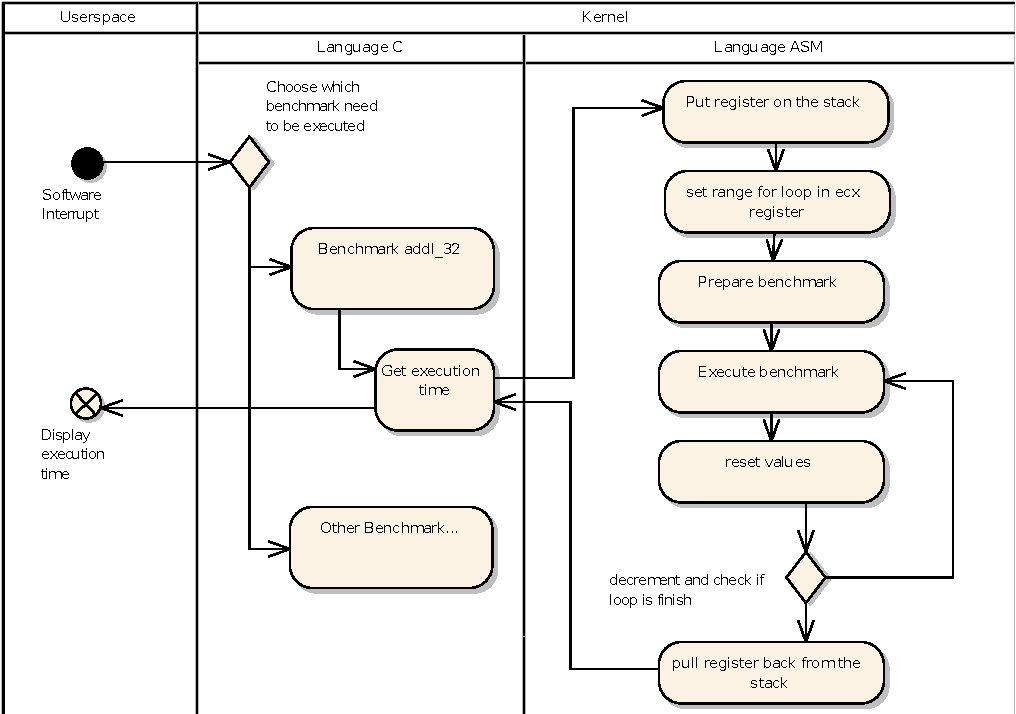
\includegraphics[width=1.0\textwidth]{images/interrupt_ea.pdf}
\caption{Interrupt}
\label{fig:Interrupt}
\end{figure}

\section{Starten des Benchmark über procfs}

Der Benchmark wurde in Form eines Kernelmodul für ein Linux Betriebssystem gebaut. Das Kernelmodul registriert für jeden Benchmark ein Pseudofile, das unter der Verzeichnisstruktur \texttt{/proc/benchmark/} abrufbar ist.
\par
Das \texttt{procfs} oder \texttt{proc filesystem} genannter Filesystem erstellt eine Schnittstelle zwischen dem Benutzermodus und dem Kernelmodus. Es ist ein virtuelles Filesystem, dass unter der Verzeichnisstruktur \texttt{/proc} gemountet wurde\cite{mauerer2010professional}. Die Dateien die sich darin befinden sind Pseudofiles. Sie sind virtuelle, weil sie nicht wirklich existieren und somit auch nicht auf ein Medium gespeichert sind. Beim schreiben beziehungsweise lesen werden die Information am Kernel weiter gegeben, verarbeitet und zurück zum lesen gestellt. Weil das verhalten der Schnittstelle einer Datei entspricht, können für die Lese- und Schreiboperation, die Linux Standart-Werkzeuge verwendet werden.


\lstset{language=bash}
\begin{lstlisting}[label={list:read_procfs},caption={Lesen im procfs}]
sriolo@desktop ~ $ cat /proc/uptime 
571433.06 1229766.89
\end{lstlisting}
\begin{lstlisting}[label={list:write_procfs},caption={Schreiben im procfs}]
sriolo@desktop ~ $ echo 1 > /proc/sys/net/ipv4/conf/default/forwarding
\end{lstlisting}

Im ersten Beispiel \autoref{list:read_procfs} wird aus der Datei \texttt{uptime} gelesen, die Betriebszeit kommt als Ausgabe. Das folgende zweite Beispiel \autoref{list:write_procfs} zeigt wie in einer Datei geschrieben werden kann. Dabei wird Kernel mitgeteilt dass, er das IP-Forwarding einschalten soll. Ein ähnlicher Aufbau hat das \texttt{sys filesystem}. Die Kommunikation ist dabei schwieriger weil das Design nicht für Menschen lesbar ist, sondern für Programme im Benutzermodus. Im Gegensatz dazu kann das \texttt{procfs} mit den Standard-Werkzeuge im ASCII-Format gelesen und geschrieben werden.
\par
Das \texttt{procfs} ist an dieser Stelle wichtig, weil der Benchmark im Kernelmodus laufen muss. Durch den Befehl \texttt{cat} auf die entsprechende Datei des Benchmark, startet im Kernelmodus den Ablauf für die Messung und gibt die verwendete Zeit als Ausgabe an. Das folgende Beispiel in \autoref{list:start_benchmark} zeigt wie der Benchmark gestartet wird und der CPU durch eine Addieroperation ausgelastet wird.

\begin{lstlisting}[label={list:start_benchmark},caption={Starten des Benchmark}]
root@galileo ~ $ cat /proc/benchmark/addl_32
321
\end{lstlisting}


\section{Aufbau der Software für die Messung}


\subsection{Grundaufbau und Ablauf eines Benchmark}
Der Grundbau der Software wurde mit der Programmiersprache C geschrieben. Der Kern des Benchmark besteht aus wenige Assembler Befehlssätze. Der Kernelmodul beinhaltet alle in dieser Arbeit relevante Benchmarks. Die \autoref{fig:Benchmark} zeigt der Ablauf des Programm.

\begin{figure}[H]
\centering
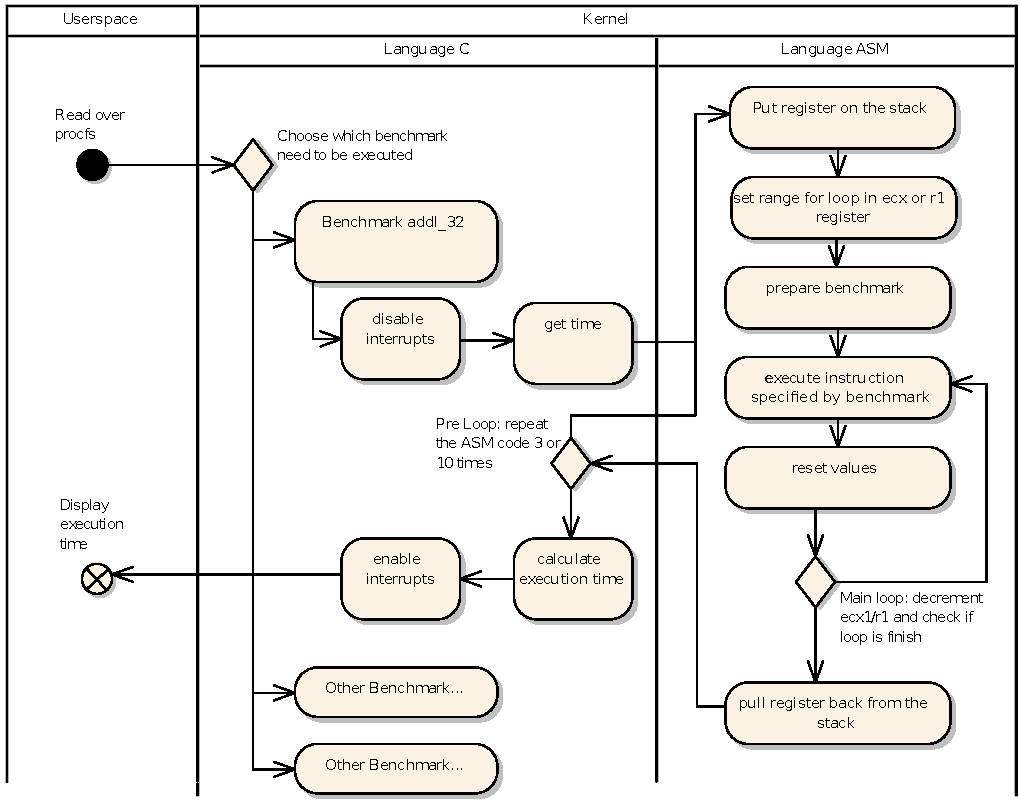
\includegraphics[width=1.0\textwidth]{images/benchmark_ea.pdf}
\caption{Benchmark}
\label{fig:Benchmark}
\end{figure}


Durch ein Systemcall, dass über das \texttt{procfs} ausgelöst wird, wird der Benchmark gestartet. Da sich in der Software mehrere Benchmark befinden muss zuerst der Benchmark ermittelt werden. An dieser Stelle werden durch die Funktion \texttt{local\_irq\_save} alle weitere Interrupts geblockt. Die Startzeit wird ermittelt und zwischen gespeichert. Das Programm wechselt zum eigentlichen Benchmark der in Assembler geschrieben ist. Ist der Assembler-Teil abgearbeitet, wird die Zeit errechnet die zur Durchführung verwendet worden ist. Durch den Aufruf der Funktion \texttt{local\_irq\_restore} wird die Blockierung von weiteren Interrupts wieder freigeben. Als letztes wird die beanspruchte Zeit im Systemcall zurück geliefert.

\lstset{language=[x64]Assembler}
\begin{lstlisting}[label={list:asm_benchmark},caption={Benchmark in Assembler}]
benchmark_imull_zero:
  stmfd    sp!, {r0-r5}
  ldr r1, = 2147483648
  ldr r3, = 0x0
  ldr r4, = 0x0
loop_benchmark_imull_zero:
  mul r5, r3, r4
  sub r1, r1, #1
  cmp r1, #0
  bge loop_benchmark_imull_zero
  ldmfd    sp!, {r0-r5}
  bx  lr
\end{lstlisting}

In der \autoref{list:asm_benchmark} ist der Assemblercode aufgeführt der, den CPU über eine länger Zeit durch die Rechenoperation $0*0$ stresst. Die \autoref{list:asm_benchmark} dient als Beispiel für den Grundbau. Auf dieser basieren dann, die unterschiedlichen Benchmarks, die je ein Befehlssatz beinhalten, der gegenüber den anderen Verglichen werden kann. Der Prozessor startet bei Zeile 1 und nächster Schritt werden alle Register \texttt{r1} bis \texttt{r5} im RAM auf einem Stack gelegt. Das Register \texttt{r1} wird mit $2^{31}$ abgefüllt. Dieser dient uns später eine Schlaufe zu erzeugen. Auf Zeile 4 und 5 wird der Benchmark auf die Rechenoperation vorbereitet, wobei \texttt{r3} und \texttt{r4} mit der Zahl 0 abgefüllt werden. Der Prozessor geht nun auf die wichtigste Zeile 7. An dieser stelle befindet sich die Multiplikation-Operation die eine Veränderung des Energieverbrauch erzeugt und gemessen wird. Nach der Abarbeitung wird der Index in Register \texttt{r1} um eins dekrementiert und anschliessend überprüft ob der Index bereits Null erreicht hat. Falls der Index noch nicht auf Null ist wird ein Programmsprung auf Zeile 7 erzeugt und die Schleife noch einmal wiederholt. Falls der Index Null erreicht hat wird der Programmsprung nicht erzeugt und dies führt zu einem austritt der Schleife. Die Register  \texttt{r1} bis \texttt{r5}, die am Anfang auf dem Stack gelegt wurden, werden aus dem RAM geholt und wiederherstellt. Damit ist das Assemblerprogramm am Ende.
\par
In der \autoref{list:asm_benchmark} wird ersichtlich das mehrere Befehlssätze nötig sind um eine Schleife zu erstellen. Obwohl nur die Zeile 7 für den Benchmark relevant ist, sind die Zeilen 8, 9 und 10 unausweichlich und verfälschen das Messresultat. Damit ein Vergleich zwischen unterschiedlichen Benchmark erstellt werden kann. Muss der Grundbau immer gleich sein. Somit ist die Messung zwar Falsch aber immer mit dem gleichem Fehler und Vergleich zwischen den Benchmarks können erstellt werden.


\subsection{Kompilation und Programmstruktur}

\begin{wrapfigure}{!}{0.7\textwidth}
\centering
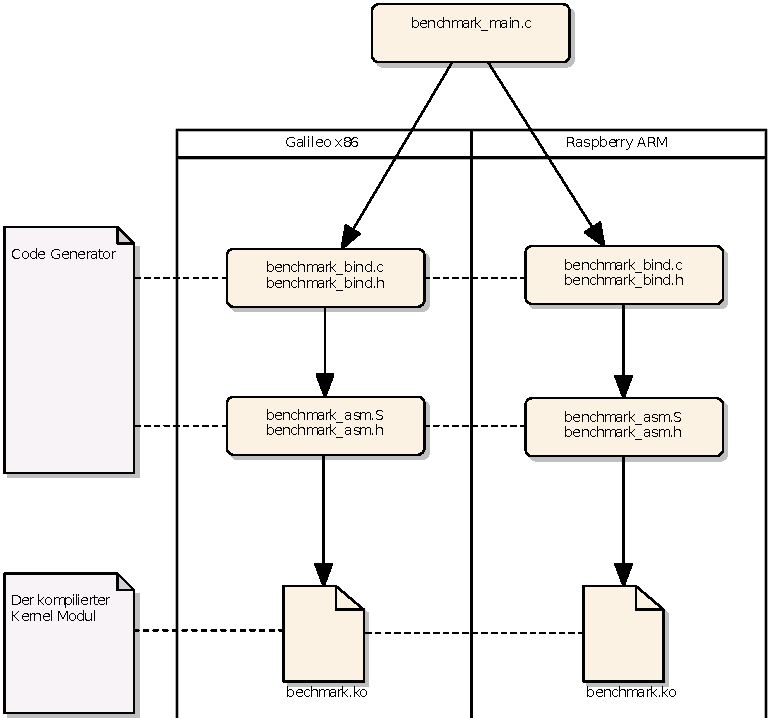
\includegraphics[scale=0.8]{images/filestructure.pdf}
\caption{Dateistruktur}
\label{fig:filestructure}
\end{wrapfigure}


Der Grundbau des Benchmark ist für jede Messung immer gleich. Deshalb wurde ein Code-Generator in Python geschrieben der für jeden Benchmark automatisch die Grundstruktur erstellt und der Inhalt aus einem Konfiguration übernimmt. Der Code-Generator wird automatisch vor dem kompilieren gestartet und die Dateien am Richtigen geschrieben damit sie der GCC kompilieren kann und anschliessen in den Kernel verlinkt werden. Die Grundstruktur des Kernel Modul liegt in der Datei \texttt{benchmark\_main.c}. Die Datei \texttt{benchmark\_bind.c} sorgt für den Übergang zum Assemblercode der sich in die Datei \texttt{benchmark\_asm.S} befindet.
\par
Der Compiler muss die Headerfiles des Kernel während des Kompiliervorgang kennen. Die Headerfiles sind aber nicht in jeder Linuxdistribution enthalten. Deswegen muss der gleiche Kernel als Source geladen werden und Compiliert werden. Dieser Vorgang würde auf einem Soc zu lange dauern. Deshalb wurde der Kernel und das Kernel-Modul auf eine Leistungsstärke Maschine Cross-Compiliert. Für das Raspberrypi wird zusätzlich ein modifizierter GCC benötigt, der sich auf der offizielle Seite zum Download bereit gestellt wird. Die Technische Dokumention befindet sich im Projektwiki unter  \url{https://github.com/codeix/thesis_ffhs_2016/wiki}. Nach dem fehlerfreien kompilieren des Kernel-Modul, kann dieser auf das Board kopiert werden und mit dem Befehl \texttt{insmod} in den Kernel geladen werden.

